\section{Zweiter Entwurf}
\subsection{Entwurfsziele}
Ziel des zweiten Entwurfs ist es, die Ideen aus \ref{cha:iteration_1_optimierungen} umzusetzen und sicherzustellen, dass sie den gewünschten Effekt erzielen.
Dazu wird der Beschleuniger in zwei Atome aufgeteilt, um die Datenmenge zu reduzieren, die jedes Atom halten muss.
Für die Aufteilung wird das 2-Block Spalten-orthogonale Muster verwendet (siehe \ref{cha:iteration_1_optimierungen_spaltenorthogonal}).
Außerdem wird die Standard-Rundenfunktion durch die modifizierte Rundenfunktion aus \ref{cha:iteration_1_modr} abgelöst.
Damit die Komponenten miteinander arbeiten können und die Atome Daten miteinander austauschen können, braucht es zusätzlich noch
einen Zustandsautomaten, der das Verhalten der Komponenten kontrolliert.
Die Atome sollen so klein sein wie möglich und dürfen dabei ruhig ein wenig die Ausführungszeit erhöhen.

\subsection{Aufbau}
\begin{figure}
	\center
	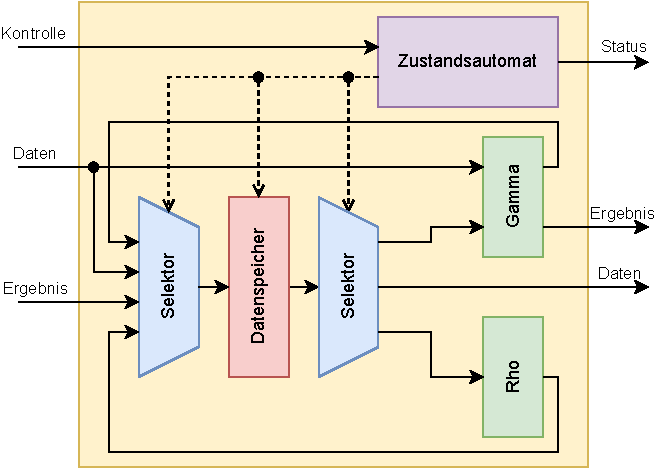
\includegraphics{images/Iteration_2.pdf}
	\caption{Atomaufbau des zweiten Entwurfs}
	\label{fig:aufbau_iteration_2}
\end{figure}
\begin{figure}
    \center
    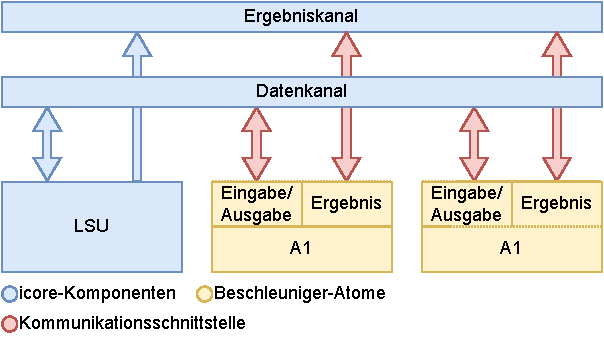
\includegraphics{images/Iteration_2_Integration.pdf}
    \caption{Integration des zweiten Beschleunigers in den icore}
    Unbenutzte Komponenten, Kontrollsignale, sowie die beiden nicht verwendeten Kanäle des Busses wurden weggelassen
    \label{fig:iteration_2_integration}
\end{figure}
Abbildung \ref{fig:aufbau_iteration_2} zeigt den Aufbau der beiden Atome \textit{A0} und \textit{A1}.
Beide Atome teilen sich den gleichen Aufbau und bekommen ihre Rolle, den sogenannten \textit{Atom-Index}, bei der Initialisierung per Kontrollsignal mitgeteilt.
Durch die Aufteilung der Daten auf beide Atome speichert jetzt jedes Atom nur noch 13 der 25 Bits jedes Slices. Diesen Teil eines Slices nennen wir im Folgenden \textit{Tile}.
Die Speicherung der Tiles findet weiterhin in einem Flip-Flop-Register statt. Zusätzlich zu den Funktionen des Speichers aus dem ersten Entwurf bietet er noch die Möglichkeit,
Eingabedaten mit dem aktuellen Speicherinhalt über ein XODER zu kombinieren. Dadurch können weitere Blöcke direkt eingelesen werden und es muss nicht das vollständige Ergebnis
der KECCAK-p-Berechnung ausgegeben und danach die Kombination aus Ergebnis und neuen Daten wieder eingelesen werden.
Die Funktionen $\rho$ und $\gamma$ sind in ihren eigenen Komponenten implementiert.
Dabei kann der Rho-Block die komplette Funktion auf seinem Teil der Daten in einem Takt direkt berechnen. Der Gamma-Block berechnet pro Takt immer jeweils zwei Slices.
Da für die Berechnung von Gamma auf den Slices immer nur die Hälfte jedes Slices im Atom gespeichert ist, muss die andere Hälfte der Eingabedaten über den Kommunikationskanals
übertragen werden und auch die Hälfte des Ergebnisses muss wieder zurück übermittelt werden. Um das zu erlauben, wird der Kommunikationskanal in zwei 32-Bit breite Teile eingeteilt.
Der Datenkanal übermittelt Daten direkt aus dem Speicher und der Ergebniskanal überträgt Ergebnisse der Gamma-Berechnung. Die Kanäle sind wie in Abbildung
\ref{fig:iteration_2_integration} dargestellt an den Bus der Fabric angebunden. Außerdem kann der Gamma-Block die Informationen zwischen halten, die notwendig sind,
um $\theta$ für den nächsten Slice zu berechnen. Auf diese Weise kann der Kommunikationsaufwand reduziert werden.
Über den Ausgabeselektor werden aus dem Speicher die Bits ausgewählt, welche Bits aus dem Speicher an die Berechnungseinheiten Rho und Gamma angelegt werden
und welche Bits über den Datenkanal der Kommunikationsschnittstelle ausgegeben werden. Der Eingabeselektor nimmt Daten aus dem Daten- und Ergebniskanal,
sowie den Berechnungseinheiten Gamma und Rho entgegen und bestimmt, welche Teile an den Speicher weitergeleitet werden.
Die Steuerung aller Komponenten übernimmt wieder der Zustandsautomat, der auch für die Einhaltung des Kommunikationsprotokolls zwischen den Atomen verantwortlich ist.

\subsection{Ablauf einer Berechnung}
\subsubsection{Dateneingabe}
Zum Einlesen der Daten können sowohl Daten- als auch Ergebnisbus gleichzeitig verwendet werden.
So kann die LSU in jedem Kontrollschritt jeweils eine Lane an den Bus anlegen und die Atome greifen sich die Lanes ab, die sie speichern müssen.
Die eingelesenen Lanes werden entweder direkt in den Speicher geschrieben oder über ein XODER mit dem aktuellen Speicherinhalt kombiniert,
falls es sich nicht um den ersten Block der SHA-3-Berechnung handelt.
\subsubsection{Rho}
Für die Berechnung von $\rho$ werden in jedem Atom alle Daten des Speichers gleichzeitig an den Rho-Block angelegt.
Das Ergebnis wird dann über den Eingabeselektor wieder in den Speicher übernommen. Da es sich bei $\rho$ um eine reine Permutation der Bits
in den einzelnen Lanes handelt, existiert der Rho-Block in der Implementierung gar nicht wirklich, sondern die Bits der Ausgabe werden einfach
permutiert wieder an den Selektor angelegt. Die ganze $\rho$-Funktion kann somit in einem einzigen Takt berechnet werden.

\subsubsection{Gamma}
Die Berechnung von Gamma wird in mehrere Teilschritte aufgeteilt. \textit{A0} ist dabei für die Berechnung der Slices 0 bis 31 zuständig und textit{A1}
führt die Berechnung für die Slices 32 bis 63 durch. Damit ein neuer Slice berechnet werden kann, muss der vollständige Slice,
sowie ein paar Informationen aus seinem Vorgänger im Atom vorliegen. Da für jeden Slice nur ein Tile im Speicher des zuständigen Atoms vorliegt,
muss das andere Tile noch übertragen werden. Das geschieht über den Datenkanal zwischen den Atomen. Bevor die Berechnung aller Slices startet,
werden die Slices 31 und 63 einmal ausgetauscht, da diese benötigt werden, um die Slices 0 und 32 zu berechnen. Für die restlichen Slices
werden diese benötigten Daten immer im Takt vorher berechnet und können kurz in der Komponente gepuffert werden.
Nach der Berechnung eines Slices muss das Ergebnis auch in beiden Atomen wieder übernommen werden. Dafür wird wieder ein Tile in den lokalen Speicher übernommen
und das andere Tile wird über den Ergebniskanal an das andere Atom übertragen und dort gespeichert. In jedem Takt können somit insgesamt vier Slices gleichzeitig berechnet werden.
Hier ist die genaue Abarbeitungsreihenfolge für einen Slice nochmal für textit{A0} beschrieben. Jeder Punkt beschreibt dabei, was in einem Takt passiert:
\begin{enumerate}
\item Die Daten für textit{A1} werden aus dem Datenspeicher gelesen und an den Datenkanal angelegt.
\item Die Daten für textit{A1} befinden sich im Register des Datenkanals
\item Die Daten für textit{A1} sind bei textit{A1} eingetroffen. Gleichzeitig treffen auch die von textit{A1} gesendeten Daten bei textit{A0} ein.
Die erhaltenen Daten werden mit den Daten aus dem Speicher von textit{A0} zu vollständigen Slices kombiniert und der Berechnungseinheit bereitgestellt.
\item Die Berechnungseinheit berechnet das Ergebnis und gibt es aus.
\item Das Ergebnis wird in zwei Tiles aufgeteilt. Eines wird im Datenspeicher übernommen und das andere wird am Ergebniskanal angelegt.
\item Das Ergebnis im Ergebnisbus befinden sich im Register des Ergebniskanals
\item Das Ergebnis trifft bei textit{A1} ein. Gleichzeitig trifft auch das Ergebnis von textit{A1} bei textit{A0} ein.
Das erhaltene Ergebnis wird im Datenspeicher übernommen.
\end{enumerate}
Die maximale Anzahl an Slices, die gleichzeitig in einem Atom berechnet werden kann, ergibt sich in diesem Fall aus der stark beschränkten Bandbreite
des Kommunikationskanals. In dem 32-Bit breiten Daten-/Ergebniskanal können maximal zwei Tiles in einem Takt übertragen werden.
Um die gesamte $\gamma$-Funktion zu berechnen, muss die oben aufgeführte Berechnungsabfolge also 16 Mal mit jeweils 2 Slices durchgeführt werden.
Die Berechnung der 7 Schritte wird in einer Pipeline durchgeführt, die zweite Berechnungsabfolge beginnt also nicht erst, wenn die erste Abfolge abgeschlossen ist,
sondern direkt, nachdem der erste Schritt der vorherigen Abfolge abgeschlossen ist. Dadurch beträgt die Berechnungsdauer aller 16 Ausführungen
$7 + (16 - 1) = 22$ Schritte. Dabei ist allerdings der Synchronisationsaufwand, wie zum Beispiel der Austausch der Slices 31 und 63, nicht enthalten.

\subsection{Bewertung}
Die Ausführungszeit für eine Iteration der modifizierten Rundenfunktion ist mit einem Faktor von 20 wie erwartet deutlich langsamer als die Implementierung des ersten Entwurfs.
Dies ist wie bereits erklärt hauptsächlich der Aufteilung der Gamma-Funktion in 16 Teilschritte geschuldet, sowie der damit einhergehenden Verzögerung.
Anders jedoch als erwartet, ist die Größe der Atome durch das Aufteilen der Berechnung und des Datenspeichers nicht wie gewünscht gesunken.
Tatsächlich ist der Entwurf mit seinen 4643 LUTs nochmal um gut 40\% größer. Dafür gibt es zwei wesentliche Gründe: den Zustandsautomaten
sowie die Komplexität der Speicherzugriffsmuster, die in der Überlegung für das Design nicht bedacht wurden.

\subsubsection{Zustandsautomat}
Der Zustandsautomat besteht aus einem Iterator, der in jedem Takt hochgezählt wird und anhand dessen die Steuersignale für die anderen Komponenten generiert werden.
Entgegen der ursprünglichen Annahme, dass seine Größe aufgrund der Einfachheit der Aufgabe vernachlässigbar ist, nimmt er in diesem Design über 300 LUTs,
also etwa 20\% der Maximalgröße von 1600 LUTs ein. Auch wenn sich die konkrete Implementierung noch optimieren lässt, so ist klar geworden,
dass die weitere Erhöhung der Berechnungskomplexität mit Bedacht durchgeführt werden muss, da der Zustandsautomat dadurch nur noch größer wird.

\subsubsection{Schreib- und Lesemuster}
Im ersten Entwurf wird der Wert jedes Bits im Register entweder von der Eingabe oder von der Ausgabe der Rundenfunktion bestimmt.
Im zweiten Entwurf hingegen hängt dieser Wert ab von der Eingabe, des Ergebnisses des Rho-Blocks, des lokalen Ergebnisses des Gamma-Blocks, sowie einem Bit im Ergebnis-Kanal.
Welches Bit aus dem Ergebniskanal für ein Bit im Datenspeicher bestimmt ist, legen der Zustandsautomat und der Atom-Index fest.
Diese Auswahlschaltung benötigt schon mehr Platz als die Reduktion der Datenmenge einspart.
Analog ist auch das Lesen der Daten komplizierter geworden. Für den Gamma-Block und den Datenkanal müssen
anhand des aktuellen Zustands und des Atom-Indexes aus allen 800 gespeicherten Bits immer ein paar auswählen.

\subsubsection{Gamma-Funktion}
Der Gamma-Block übernimmt praktisch den gesamten Rechenaufwand der modifizierten Rundenfunktion. Da die Berechnung auf
zwei Atome aufgeteilt ist und auch nicht alle Slices in einem Atom gleichzeitig berechnet werden, ist der Platzbedarf für
die $\gamma$-Berechnung sehr stark geschrumpft, sodass das aktuelle Design nur etwa 70 LUTs benötigt.
Eine weitere Optimierung der Berechnungsweise von $\gamma$ ist daher auch in weiteren Iterationen nicht mehr nötig.

\subsection{Optimierungsansätze}
Die starke Steigerung der Speicherkomplexität ist das Hauptproblem des Entwurfs und weitere Verbesserungen müssen hier ansetzen,
um den Beschleuniger aus die erforderliche Größe reduzieren zu können. Um die Speicherverwaltung vollständig aus dem Design zu entfernen,
hatten wir die Nutzung der BRAM-Blöcke in den Überlegungen des ersten Entwurfs schon einmal in Erwägung gezogen und uns letztendlich dagegen entschieden,
weil die Verwendung des BRAM das Festlegen auf eine feste Orientierung der gespeicherten Daten bedeutet. Damit der Gamma-Block einfach wiederverwendet werden kann,
ist es sinnvoll, die aktuelle Aufteilung der Daten zu berücksichtigen. Die einzig sinnvolle Orientierung des Speichers ist somit Lane-orthogonal,
Also Daten werden immer als ein ganzzahliges Vielfaches an Tiles gespeichert. So können immer ganze Tiles dem Gamma-Block bereitgestellt werden.
Da die Rho-Funktion, eigentlich auf Lanes arbeitet, muss dann aber in ihrer Implementierung so angepasst werden, dass sie mit Tiles arbeiten kann.

\subsubsection{Transformation der Rho-Funktion}
\label{cha:iteration_2_rho_transformation}
Das Berechnen der Rho-Funktion auf Tile orientierten Daten kann mit Hilfe mehrerer Schieberegister realisiert werden.
Dazu wird die Berechnung in zwei Stufen aufgeteilt. Die erste Stufe berechnet Links-Rotationen um maximal 32 Bits
und die zweite Stufe berechnet Rechts-Rotationen um maximal 32 Bits. Mit der aktuellen Aufteilung der Daten müssen in beiden Atomen
maximal sieben Links- bzw. Rechts-Rotationen gleichzeitig durchgeführt werden. Da die Berechnungen der Lanes untereinander unabhängig sind,
können wir einfach eine Lösung für eine einzelne Lane siebenmal nebeneinander implementieren. Sollte der Platz dafür nicht ausreichen,
kann die Berechnung auch in noch mehr als zwei Stufen eingeteilt werden, was zwar nochmal mehr Berechnungszeit, dafür aber weniger Platz benötigt.
Der Pseudocode \ref{fig:iteration_2_leftshift} skizziert, wie eine Links-Rotation einer Lane um eine fixe Distanz $k <= 32$ mit Hilfe eines 32-Bit Schieberegisters
durchgeführt werden kann.
\begin{figure}
\lstset{language=C}
\begin{lstlisting}[label={lst:shift_left}]
Lane shift_left(Lane x, Distance k)
{
  lane result = 0
  Bit[32] buffer           // Unser Schieberegister, das nur
                           // mit << 1 geschoben werden darf.
  
  for i in 32 to 63 {      // Die oberen 32 Bits der Lane
    buffer = buffer << 1   // werden nach und nach in den
    buffer[0] = x[i]       // Puffer geschrieben
  }
  
  for i in 0 to 63 {       // Aus dem Puffer kann dann
    r[i] = buffer[k]       // immer an der gleichen Stelle
    buffer = buffer << 1   // ein Ergebnisbit ausgelesen werden
    buffer[0] = x[i]
  }
  return result
}
\end{lstlisting}
\caption{Pseudocode für die Berechnung einer Links-Rotation mit Hilfe eines Schieberegisters}
\label{fig:iteration_2_leftshift}
\end{figure}
Die Rechts-Rotation funktioniert genau analog, nur werden die Ein- und Ausgabebits in der anderen Reihenfolge eingelesen / geschrieben;
Mit diesem Vorgehen kann jede beliebige Rotation um 32 Bits mit nur einem Puffer realisiert werden, wobei jede unterschiedliche
Distanz ein anderes Bit aus dem Puffer auswählt. Außerdem können auch immer mehrere Bits gleichzeitig gelesen und geschrieben werden,
indem der Inhalt des Schieberegisters um mehr als eine Stelle pro Schritt bewegt wird.
Maximal brauchen wir von diesen Registern sieben Stück. Je mehr sich in den Beschleuniger integrieren lassen,
desto schneller ist die Berechnung der $\rho$-Funktion. Da die zu lesenden und zu schreibenden Bits jedes Schritts nicht von der Rotations-Distanz
abhängen, befinden für mehrere Puffer alle benötigten / berechneten Bits immer in den gleichen Tiles.
Somit funktioniert die ganze Berechnung auf Slice-orientierten Daten.

\subsubsection{BRAM als Datenspeicher}
Mit dem neuen Ansatz für die Berechnung der $\rho$-Funktion kann auch der Datenspeicher in den BRAM verschoben werden,
da das Problem der unterschiedlichen Ausrichtung der benötigten Eingabedaten behoben ist. Ein BRAM Block unterstütz
dabei bis zu zwei Lese- und Schreibports. Das ist essenziell für die Berechnung der $\gamma$-Funkion,
da durch die Pipeline in jedem Takt sowohl Daten für die eigenen Berechnungen, als auch für die Berechnungen des
jeweils anderen Atoms gelesen werden müssen und auch die Ergebnisse beider Atome gleichzeitig festgehalten werden müssen.
Da der Gamma-Block immer zwei Slices gleichzeitig verarbeitet, bietet sich dieses Format auch für die Breite der Speicherports an.
So können von jedem Port immer zwei Tiles gleichzeitig adressiert werden. Da jeder Atom Contrainer über insgesamt 3 BRAM Einheiten verfügt,
können die Ergebnisse der $\gamma$-Funktion auch in einer anderen Einheit gespeichert werden als die Eingabedaten.
Die $\rho$-Funktion kann tatsächlich quasi inplace in einem BRAM-Block berechnet werden, da der BRAM read-before-write-Zugriffe unterstützt.
Wird ein Tile k gelesen und liegt das Ergebnis n Takte später vor, so kann es an der Stelle k + n gespeichert werden,
nachdem im gleichen Takt der alte Slice mit dem Index k + n gelesen wurde. Das bedeutet, dass beide Ports gleichzeitig
Daten für die Berechnung bereitstellen können, sodass immer 4 Tiles gleichzeitig in den Puffer eingelesen werden können.
Auf diese Weise benötigt die Berechnung einer vollständigen Rotation somit theoretisch etwa 8 Takte zum Füllen des Puffers mit den Initialwerten
und 16 Takte zum Lesen Schreiben aller Tiles zuzüglich zu ein paar Verzögerungstakten aufgrund des BRAMs.

\subsubsection{Datenbus}
Da sowohl der Gamma-Block als auch der neue Rho-Block in Zusammenarbeit mit dem BRAM wie oben beschrieben
niemals auf mehr als zwei Ports gleichzeitig lesen oder schreiben,
können die Datenleitungen für immer jeweils zwei Ports auf unterschiedlichen BRAM-Einheiten zusammengelegt werden.
Wie das genau aussieht, ist im nächsten Kapitel genauer erläutert.